\documentclass[main.tex]{subfiles}
\begin{document}

\section{Интерпретации квантовой механики}\label{ch3}

Эта книга не будет включать в себя исчерпывающее обсуждение всех предлагаемых интерпретаций того, чем на самом деле является квантовая механика. Существующие подходы подробно описаны в литературе [1, 68, 10, 11, 35], но мы думаем, что все они содержат слабые стороны. Наиболее консервативный из них - копенгагенская интерпретация. Она очень прагматична, и некоторые ведущие исследователи настаивают на том, что она содержит все, что нам нужно знать о квантовой механике.

Все же есть вещи, которые не объясняются в картине Копенгагена. Ниже мы покажем, как интерпретация клеточного автомата решит некоторые из этих вопросов.


\subsection{Копенгагенская доктрина}\label{ch3.1}

Должно быть, это был очень волнующий период ранней современной науки, когда исследователи начали понимать, как обращаться с квантовой механикой, в конце 1920-х и последующих годах [64]. Копенгагенская доктрина - это первая связная картина того, как нужно думать о квантовой механике. На начальном этапе физики по большей части боролись с уравнениями и техническими трудностями. Сегодня мы точно знаем, как с этим справиться, и теперь мы можем гораздо точнее перефразировать исходные отправные точки. Первоначально квантовая механика была сформулирована в терминах волновых функций, с помощью которых можно было описать состояния электронов; игнорируя спин, имеем стандартную форму: $\psi(\vec x, t) = \langle\vec x\mid\psi(t)\rangle$. Теперь мы можем использовать слова ``волновая функция'', когда действительно хотим говорить о кет-состояниях в более общих терминах.

Не заостряясь на том, кто именно и что сказал в 1920-х годах, раскроем основные моменты копенгагенской доктрины. Несколько анахронично,\footnote{Позвольте мне здесь еще раз подчеркнуть, что из нашего использования таких терминов, как "копенгагенская интерпретация" или "Копенгагенская доктрина", не следует делать вывод, что наши описания будут попытками переписать историю; философские дебаты, которые действительно имели место среди "Копенгагенской группы", кем бы они ни были на самом деле, были довольно сложными и разнообразными. Здесь мы просто используем эти фразы для характеристики одного конкретного общего отношения к квантовой механике.} мы используем обозначение Дирака:

\textit{Система полностью описывается своей ``волновой функцией'', которая является элементом гильбертова пространства, и любой базис в гильбертовом пространстве может быть использован для ее описания. Эта волновая функция подчиняется линейному дифференциальному уравнению первого порядка во времени, которое называется уравнением Шредингера, точная форма которого может быть определена путем  экспериментов.}

Измерение может быть выполнено с использованием любой наблюдаемой $\mathcal{O}$, которой можно поставить в соответствие эрмитовый оператор в гильбертовом пространстве. Затем теория предсказывает, что среднее измеренное значение $\mathcal{O}$ после многих повторений эксперимента будет

\begin{equation}\label{3.1}
	\langle\mathcal{O}\rangle=\langle\psi(t)|\mathcal{O}| \psi(t)\rangle
\end{equation}

Как только измерение выполнено, волновая функция системы коллапсирует до состояния в подпространстве гильбертова пространства, которое является собственным состоянием наблюдаемой $\mathcal{O}$, или вероятностным распределением собственных состояний, согласно формуле (\ref{3.1}).

Когда две наблюдаемые $\mathcal{O}_1$ и $\mathcal{O}_2$ не коммутируют, они не могут быть точно измерены одновременно. Коммутатор [$\mathcal{O}_1$, $\mathcal{O}_2$] указывает, насколько большим может быть произведение ``неопределенностей'' $\delta\mathcal{O}_1$ и $\delta\mathcal{O}_2$. Само измерительное устройство должно рассматриваться как классический объект, а для больших систем квантово-механическое измерение приближается к классическому описанию.

В формулу (\ref{3.1}) неявно включены елементы вероятности. Если мы расширим волновую функцию $\left | \psi \right>$ на собственные состояния $\left | \varphi \right>$ наблюдаемой $\mathcal{O}$, то мы обнаружим, что вероятность того, что эксперимент на выявление $\left | \psi \right>$ фактически дает в результате нахождение собственного значения состояния $\left | \varphi \right>$, будет равна $P = \left| \langle\varphi\mid\psi\rangle \right|^2$. Это называется правилом вероятности Борна [12, 13].

Отметим, что волновой функции не может быть придано никакого онтологического значения. Не требуется существование никакой ``пилотной волны''; на самом деле нельзя измерить $\langle\varphi\mid\psi\rangle$ само по себе; только с помощью повторных экспериментов можно измерить вероятности с внутренними границами погрешности. Мы говорим, что волновая функция, или, точнее, амплитуды, скорее пси-эпистемологические, чем пси-онтические.

Важным элементом копенгагенской интерпретации является то, что можно \textit{только спросить, каким будет результат эксперимента}. В частности, запрещено спрашивать: что на самом деле происходит? Именно последний вопрос вызывает бесконечные дискуссии; Важный момент, сделанный копенгагенской группой, заключается в том, что такие вопросы не нужны. Если кто-то знает уравнение Шредингера, он знает все, что нужно для предсказания результатов эксперимента, больше не нужно задавать никаких вопросов.

Это сильная сторона копенгагенской доктрины, но она также накладывает серьезные ограничения. Если мы знаем уравнение Шредингера, мы знаем все, что нужно знать; однако, что если мы еще не знаем уравнения Шредингера? Как прийти к правильному уравнению? В частности, как мы можем прийти к правильному гамильтониану, если задействована сила гравитации?

Гравитация была главным объектом внимания последних 30 лет и в теории элементарных частиц и в теории пространства и времени. Было выдвинуто много догадок, порой совсем диких. В частности, (супер)теория струн добилась огромных успехов. Тем не менее, не была построена ни одна убедительная модель, которая объединяет гравитацию с другими силами; Предложенные модели не могут вменяемо объяснить, не говоря уже о прогнозировании, значения фундаментальных констант Природы, включая массы многих фундаментальных частиц, постоянную тонкой структуры и космологическую постоянную. И вот здесь, по мнению автора, мы должны спросить: что на самом деле происходит или что это может быть?

Одной из сильных особенностей копенгагенского подхода к квантовой теории было то, что было также ясно показано, как можно получить уравнение Шредингера, если известен классический предел:

\textit{Если классическая система описывается (непрерывными) уравнениями Гамильтона, это означает, что у нас есть классические переменные $p_i$ и $q_i$, для которых можно определить скобки Пуассона. Заменив их коммутаторами, мы получаем квантовую модель, классический предел которой ($\hbar\rightarrow 0$) соответствует данной классической системе.}

Это очень мощный трюк, но, к сожалению, в случае гравитационной силы он недостаточно хорош, чтобы дать нам ``квантовую гравитацию''. Проблема гравитации заключается не только в том, что гравитационная сила кажется не перенормируемой или что трудно определить квантовые версии пространственно-временных координат, а также в физических аспектах нетривиальных топологий пространства-времени; некоторые авторы пытаются решить эти проблемы как чисто технические, которые можно решить с помощью некоторых приемов. Реальная проблема заключается в том, что кривизна пространства-времени выходит из-под контроля в масштабе Планка. Мы будем вынуждены обратиться к другой системе законов для физических степеней свободы Природы.

Перспективным подходом было использование локальной конформной симметрии [59, 111, 112] в качестве более фундаментального принципа, чем считается обычно; это может быть способом сделать шкалы расстояний и времени относительными, чтобы то, что называется ``небольшими расстояниями'', перестало иметь абсолютное значение. Теория повторяется в Приложении B. Она действительно нуждается в дальнейшей полировке, и это также может в конечном итоге потребовать интерпретацию клеточного автомата для некоторых квантовых свойств.

\subsection{Точка зрения Эйнштейнианца}\label{ch3.2}

    
Этот раздел называется ``точка зрения Эйнштейнианца'', а не ``точка зрения Эйнштейна'', потому что мы не хотим вдаваться в дискуссию о том, что на самом деле думал Эйнштейн. Хорошо известно, что Эйнштейн был не в восторге от копенгагенской доктрины. Идея о том, что можно сформулировать теорию, в которой все явления во Вселенной контролируются уравнениями, которые не оставляют ничего случайного, теперь будет называться эйнштейновским взглядом. Мы задаем дополнительные вопросы, такие как: Можно ли считать квантово-механическое описание физической реальности полным? [33, 53], или теория говорит нам то, что мы хотели бы знать об окружающих явлениях?

В мысленном экспеименте Эйнштейна-Подольского-Розена две частицы (например, фотоны) создаются в состоянии

\begin{align}\label{3.2}
	x_1 - x_2 = 0, &&
	p_1 + p_2 = 0
\end{align}

Поскольку $[x_1 - x_2, p_1 + p_2] = 0$, оба уравнения в (\ref{3.2}) могут выполняться одновременно.

Что действительно беспокоило Эйнштейна, Подольского и Розена, так это то, что спустя много времени после того, как две частицы перестали взаимодействовать, наблюдатель частицы № 2 мог бы решить либо измерить ее импульс $p_2$, после чего мы точно знаем импульс $p_1$ частицы №1, либо положение $x_2$, после которого мы бы точно знали положение $x_1$ частицы №1. Как такая частица может быть описана квантово-механической волновой функцией вообще? Очевидно, измерение на частице №2 повлияло на состояние частицы №1, но как это могло произойти?

Однако в современной квантовой терминологии мы бы сказали, что измерения, предложенные в этом мысленном эксперименте, нарушили бы волновую функцию запутанных частиц. Измерения на частице №2 влияют на распределения вероятностей для частицы №1, которые никоим образом не должны рассматриваться как эффект появления сигнала от одной системы на другую.

В любом случае, даже Эйнштейн, Подольский и Розен не испытывали затруднений при вычислении квантово-механических вероятностей для результатов измерений, так что в принципе квантовая механика выходила невредимой из этой последовательности аргументов.

Гораздо сложнее описать два фотона ЭПР в классической модели. Такие вопросы будут темой разд.\ref{ch3.6}.

У Эйнштейна возникли трудности с релятивистской инвариантностью квантовой механики (``есть ли ужасная информация, передаваемая этими частицами быстрее света?''). Теперь это рассматривается как технические трудности, которые уже решены. Копенгагенская доктрина подразумевает, что передача информации на расстоянии может иметь место, только если мы можем идентифицировать некоммутирующие операторы $A$ в точке $x_1$ пространства-времени и $B$ в точке $x_2$ пространства-времени: $[A, B] = 0$. Теперь мы понимаем, что в теории элементарных частиц все пространственно подобные разделенные наблюдаемые взаимно коммутируют, что исключает любую передачу сигналов быстрее, чем свет. Это идущая в комплекте фишка Стандартной модели, которой она во многом обязана своим успехом.

Таким образом, перейдем к более существенным эйнштейновским возражениям против копенгагенской доктрины квантовой механики: это вероятностная теория, которая не говорит нам о том, что на самом деле происходит. Иногда даже говорят, что мы должны приостановить наше ``классическое'' чувство логики. Другие возражают, дескать: ``Продолжайте помнить, что не надо задавать вопросов, изменяя свое чувство логики, и все будет хорошо.'' По мнению настоящего автора, дебаты об Эйнштейне-Боре еще не закончены. Необходимо найти теорию, которая не заставляет нас пересматривать какие-либо аспекты классического логического мышления.

Похоже, что Эйнштейн и Бор сошлись на важности роли наблюдателя. Действительно, это был важный урок, извлеченный в 20-м веке: если что-то не может наблюдаться, это, возможно, не является четко определенной концепцией - оно может даже не существовать вообще. Мы должны ограничиться наблюдаемыми особенностями теории. Это важная составляющая нашей нынешней работы, которую мы предлагаем отделить от этой доктрины, по крайней мере, до некоторой степени: вещи, которые непосредственно не наблюдаемы, могут все еще существовать и как таковые играют решающую роль в наблюдаемых свойствах объекта. Они также могут помочь нам построить реалистичные модели мира.

Действительно, существуют большие проблемы с высказыванием о том, что все, о чем мы говорим, должно быть видимо. Наблюдая за микроскопическими объектами, наблюдатель может нарушать их, даже в классической теории; Более того, в теориях гравитации наблюдатели могут нести гравитационные поля, которые нарушают систему, на которую они смотрят, поэтому мы не можем позволить себе сделать наблюдателя бесконечно тяжелым (с большими сумками, полными ``данными'', чей вес гравитационно нарушает окружающую среду), но также нельзя делать его и бесконечно легким (легкие частицы вообще не передают большие объемы данных), хотя, если масса наблюдателя будет ``где-то посередине'', это может повлечь за собой то, что наша теория будет неточной с самого начала.\footnote{Следует понимать, что наблюдатель, это не человек смотрящий в лупу и записывающий результаты в блокнотик, а некая система, которая будет обмениваться информацией с изучаемым объектом (взаимодействовать)\textit{ - Прим. перев.}}

Интересный удар был нанесен доктрине, когда была предложена теория кварков, поставив под сомнение, что наблюдаемость является центральным аспектом. Кварки не могут быть изолированы, чтобы их можно было наблюдать по отдельности, и по этой причине идея о том, что кварки будут физическими частицами, подверглась критике. К счастью, в этом случае теоретическая согласованность доказательств в пользу кварков стала настолько подавляющей, и экспериментальные методы их наблюдения, даже если они не были полностью разделены, настолько улучшились, что все сомнения испарились.

Короче говоря, Интерпретация Cellular Automaton предлагает нам вернуться к классической логике и строить модели. Эти модели описывают эволюцию больших наборов данных, что в конечном итоге может привести к классическим явлениям, которые мы можем наблюдать. Тот факт, что сами эти данные нельзя непосредственно наблюдать, и что наши эксперименты не дадут ничего, кроме статистической информации, включая флуктуации и неопределенности, можно полностью объяснить в настройках моделей; если наблюдатель больше не участвует в определении физических степеней свободы и их значений, тогда его ограниченные способности больше не будут мешать точным формализмам.

Мы подозреваем, что эта точка зрения ближе к Эйнштейну, чем к Бору, но, в некотором смысле, ни один из них не согласится полностью. Мы не претендуем на то, что наша точка зрения явно лучше, а скорее на то, что нужно пытаться идти по таким путям и учиться на наших успехах и неудачах.

\subsection{Понятия не допустимые в CAI}\label{ch3.3}

Часто пытаются придать физический смысл волновой функции сверх того, что раскрыто в классической интерпретации. Может ли она иметь онтологическое значение в качестве ``пилотной волновой функции'' [10, 11, 26]? Почти на каждой странице этой книги должно быть ясно, что мы не хотим придавать какой-либо онтологический смысл волновой функции, если мы используем ее в качестве шаблона.

В онтологическом описании нашей вселенной, с точки зрения онтологического базиса, волновая функция может принимать только два значения: 1 и 0. Состояние фактически реализуется, когда волновая функция равна 1, и оно не описывает наш мир, когда волновая функция равна нулю. Именно такую ``универсальную волновую функцию'' можно назвать \textbf{онтологической}.

Только по математическим причинам можно впоследствии захотеть снабдить эту волновую функцию фазой $e^{i\varphi}$. В онтологическом отношении эта фаза $\varphi$ вообще не имеет физического смысла, но как только рассматриваются операторы, такие как оператор эволюции времени $U(t)$ и гамильтониан, эти фазы должны быть выбраны. С физической точки зрения любая фаза так же хороша, как и любая другая, но для сохранения математической сложности под контролем, точные определения этих фаз имеют решающее значение. Затем можно выполнить унитарные преобразования для любого из базовых выборов, обычно используемых в физике. Состояния шаблонов, введенные впоследствии, имеют четко определенные фазы.

Семантическое осложнение возникает, как только мы применяем вторичное квантование. Когда одночастичное состояние описывается волновой функцией, теория вторичного квантования иногда заменяет его операторным полем. Его физический смысл тогда совершенно другой. Поля оператора, как правило, не являются онтологическими, поскольку они являются superimposables (наложенными, ...), а не beables (способные, бытийные) (см. Раздел \ref{ch2.1.1}), но в принципе они могут быть и онтологическими; Волновые функции, напротив, являются элементами гильбертова пространства, и поэтому их не следует путать с операторами, не говоря уже о beables операторах.

Формулировки так называемой ``многомировой интерпритации'' [35] квантовой механики, не всегда согласованы [29, 30]. При работе с обычной физикой атомов и элементарных частиц эта интерпретация вполне может удовлетворить основные потребности исследователя, но из того, что было изучено в этой книге, должно быть очевидно, что наша теория сильно контрастирует с такими идеями. Существует только один единственный мир, который выбирается в нашей теории как ``реальный мир'', тогда как все остальные просто не реализуются.

Читатель, возможно, заметил, что основная тема в этой книге поочередно называется ``теорией'' и ``интерпретацией''. Теория, которую мы описываем, состоит не только из предположения о том, что онтологический базис существует, но также и о том, что он может быть получен, чтобы обеспечить онтологическое описание нашей вселенной. Когда мы говорим об интерпретации, это означает, что, даже если нам трудно или невозможно идентифицировать онтологический базис, одного лишь предположения о том, что он может существовать, достаточно, чтобы помочь нам понять, чего на самом деле стоят квантово-механические выражения, обычно используемые в физике, и как можно представить себе физическую реальность, лежащую в их основе.

Есть еще один аспект нашей теории, который отличается от обычной квантовой механики; Это понятие, что наши онтологические переменные, beables, вероятно, применимы только к самым базовым степеням свободы физического мира, которые относятся к шкале Планка. Это наименьшая шкала расстояний, относящаяся к физике, и мы к ней вернемся. Совершенно не ясно, можем ли мы преобразовать онтологические переменные в те, которые все еще имеют смысл в масштабах, где физики могут проводить эксперименты сегодня, и это вполне может быть причиной того, что такие переменные практически не играют никакой роли в существующих моделях Природы, таких как Стандартная модель.

У нас есть основания подозревать, что именно по этой причине мы имеем квантовую механику, а не онтологическую теорию, описывающую известные сегодня частицы и силы: физика еще не была готова идентифицировать истинно онтологические степени свободы.

\subsection{Коллапс волновой функции и кот Шредингера}\label{ch3.4}

Следующий ингредиент в копенгагенской интерпретации, раздел \ref{ch3.1}, часто становится объектом споров:

\textit{Как только измеряется наблюдаемая величина $\mathcal O$, волновая функция системы коллапсирует до состояния в подпространстве гильбертова пространства, которое является собственным состоянием наблюдаемого $\mathcal O$, или вероятностным распределением собственных состояний.}

Это называется ``коллапсом волновой функции''. Похоже, что действие самого измерения заставляет волновую функцию принимать новую форму. Затем задается вопрос: какой физический процесс связан с этим?

Опять же, официальный ответ в соответствии с копенгагенской доктриной заключается в том, что этот вопрос не следует задавать. Сделайте расчет и проверьте свой результат с помощью экспериментов. Однако, по-видимому, существует противоречие, и это иллюстрируется мысленным экспериментом Эрвина Шредингера с кошкой [75-77]. Эксперимент сводится к следующему:

В запечатанной коробке некто выполняет типичный квантовый эксперимент. Это может быть эксперимент Штерна Герлаха, в котором частицу со спином 1/2 с ускорением направляют через неоднородное магнитное поле, которое расщепляет волновую функцию в соответствии со значениями спина в направлении $y$, или это может быть радиоактивный атом, имеющий вероятность 1/2 распада в течение определенного времени. В любом случае волновая функция хорошо определена при t = 0, а при t = 1 она находится в суперпозиции двух состояний, которые отправляются на детектор, который определяет, какое из двух состояний реализовано. Ожидается, что волновая функция «коллапсирует» в одно из двух возможных конечных состояний.

Коробка также содержит живую кошку (и воздух для того, чтобы животинка дышала). В зависимости от результата измерения, капсула с ядом разбивается или остается неповрежденной. Кошка умирает, когда обнаруживается одно состояние, в противном случае кошка остается в живых. В конце эксперимента мы открываем коробку и осматриваем кошку.

Ясно, что вероятность того, что мы найдем мертвую кошку, составляет около 1/2, а в противном случае она буде живой. Тем не менее, мы могли бы также рассмотреть эксперимент с микроскопической точки зрения. Начальное состояние было чистым, ``стандартным'', квантовым состоянием. Конечное состояние представляется смесью. Будет ли, таким образом, кошка находится в суперпозиции состояний \textit{живая} \textbf{и} \textit{мертвая}?

Аксиома коллапса говорит нам, что состояние  должно представляться ``мертвым котом'' \textit{или} ``живым котом'', в то время как ранерасмотренное описание квантовых механических состояний гильбертова пространства явно диктует, что если в квантовой системе возможны два состояния, $\left|\psi_1\right>$ и $\left|\psi_2\right>$, тогда мы также можем получить $\alpha\left|\psi_1\right> + \beta\left|\psi_2\right>$. Согласно уравнению Шредингера, эта суперпозиция состояний всегда превращается в суперпозицию конечных состояний. Коллапс, кажется, нарушает уравнение Шредингера. Что-то выходит не совсем правильно.

Ответ, предложенный некоторыми исследователями [65, 66], заключается в том, что, по-видимому, уравнение Шредингера является лишь приближенным, и что крошечные нелинейные ``поправочные члены'' приводят к коллапсу [4, 41, 73]. Одна из проблем заключается в том, что наблюдения могут проводиться в совершенно разных масштабах пространства, времени, энергии и массы. Насколько большими должны быть предполагаемые условия коррекции? Во-вторых, как поправочные слагаемые заранее знают, какие измерения мы планируем выполнить?

Некоторые авторы пытаются приписать разделение состояния мертвой кошки и состояния живой кошки ``декогеренции''. Но тогда что такое декогеренция? Почему мы не можем рассмотреть всю коробку с кошкой в ней, в полной изоляции от окружающей среды?

Мы полагаем, что именно здесь на помощь придет КА-интерпретация квантовой механики. Она сформулирована без использования волновой функции, но вместо этого существуют онтологические состояния. В итоге получается только одна волновая функция, которая принимает значение 1, если у нас есть состояние, в котором находится вселенная, и 0, если это состояние не реализовано. Нет других волновых функций, нет суперпозиции.

Как это объясняет феномен коллапса, будет объяснено в гл.\ref{ch4}. Вывод: квантовая механика - не базовая теория, а инструмент для решения математических уравнений. Этот инструмент работает так же хорошо для наложенных состояний (шаблонов), как и для онтологических состояний, но это не одно и то же. Мертвый кот находится в онтологическом состоянии, как и живой. Для наложенного (superimposed) кота уравнения решаются математически вполне приемлемым способом, но он не описывается состоянием, которое может возникнуть в реальном мире. Мы отложим точное объяснение до гл. \ref{ch4}. Это будет звучать очень странно для физиков, которые выросли на стандартной квантовой механике, но это обеспечивает логическое решение парадокса кота Шредингера.\footnote{Критично настроенные читатели возразят: конечно, эта теория не является квантовой механикой, поэтому она не разделяет ни одной из ее проблем. Верно, но наша теория должна генерировать квантовую механику, не создавая связанных с ней проблем.}

Кто-нибудь может спросить, что может означать случай, когда у нас есть преобразования между онтологическими состояниями и шаблонными состояниями. Наш опыт говорит нам, что все состояния шаблона, которые являются суперпозициями $\alpha\left|\psi_1\right> + \beta\left|\psi_2\right>$ онтологических состояний, могут служить подходящими приближениями, описывающими вероятностные ситуации в реальном мире. Как может случиться так, что иногда они кажутся онтологическими? Наиболее вероятным ответом на это будет то, что преобразование не всегда должно быть полностью локальным, но на практике может включать в себя множество состояний зрителя в окружающей среде. В чем мы можем быть уверены, так это в том, что все онтологические состояния образуют ортонормированное множество. Таким образом, всякий раз, когда мы используем $\alpha\left|\psi_1\right> + \beta\left|\psi_2\right>$ для описания онтологического состояния, в среде должны присутствовать другие волновые функции, которые должны выбираться по-разному для любой отдельной пары $\alpha$ и $\beta$, так что весь набор, который мы используем для описания физических ситуаций всегда ортонормирован.

Это следует учитывать в следующих разделах, где мы комментируем мысленные эксперименты с Алисой и Бобом.

В работе [96] утверждается, что аксиома коллапса в традиционных описаниях квантовой механики, по существу, приводит к необходимости существования предпочтительного ортонормированного набора базисных состояний. Наши рассуждения противоположны: мы начинаем с фундаментального ортонормированного базиса и получаем из этого коллапс волновой функции.

\subsection{Декогереция и правило Борна}\label{ch3.5}

Интерпретация клеточных автоматов устраняет один довольно мутный компонент более стандартных схем интерпретации: роль «декогеренции». Этот аргумент часто используется для объяснения того, почему макроскопические системы никогда не встречаются в квантовой суперпозиции. Пусть $\left|\psi_1\right>$ и $\left|\psi_2\right>$ два состояния, в которых может находиться классическая система, например, кошка мертва и кошка жива. Согласно Копенгагену, в своем первозданном виде квантовая механика могла бы предсказать возможность третьего состояния, $\left|\psi_3\right> = \alpha\left|\psi_1\right> + \beta\left|\psi_2\right>$, где $\alpha$ и $\beta$ могут быть любой парой комплексных чисел удовлетворяющей $|\alpha|^2 +  |\beta|^2 = 1$.

Действительно, кажется почти неизбежным, что система, которая может эволюционировать в состояние $\left|\psi_1\right>$ или в состояние $\left|\psi_2\right>$, должна также учитывать состояния, которые эволюционируют в $\left|\psi_3\right>$. Почему мы не наблюдаем такие состояния? Единственное, что мы наблюдаем - это ситуация, вероятность которой в $\left|\psi_1\right>$ может быть $|\alpha|^2$, а вероятность быть в $\left|\psi_2\right>$ равна $|\beta|^2$. Но это не то же самое, что состояние $\left|\psi_3\right>$.

Часто приводится аргумент, что состояние $\left|\psi_3\right>$ является нестабильным. Согласно Копенгагену, вероятность того, что состояние $\left|\psi\right>$ перейдет в $\left|\psi_3\right>$ будет равна

\begin{equation}\label{3.3}
	P_{3}=\left|\left\langle\psi_{3} | \psi\right\rangle\right|^{2}=|\alpha|^{2}\left|\left\langle\psi_{1} | \psi\right\rangle\right|^{2}+|\beta|^{2}\left|\left\langle\psi_{2} | \psi\right\rangle\right|^{2}+2 \operatorname{Re}\left(\alpha^{*} \beta\left\langle\psi | \psi_{1}\right\rangle\left\langle\psi_{2} | \psi\right\rangle\right)
\end{equation}

Последней слагаемое здесь отвечает за интерференцию. Это отличает настоящую квантовую теорию от классических теорий. Теперь можно сказать, что, если $\left|\psi_1\right>$ и $\left|\psi_2\right>$ становятся классическими, они не могут оставаться невосприимчивыми к взаимодействию с окружающей средой. При наличии таких взаимодействий энергии у $\left|\psi_1\right>$ и $\left|\psi_2\right>$ не будут точно совпадать, и, следовательно, интерференционный член будет сильно колебаться. Затем это слагаемое можно усреднить до нуля. Первые два слагаемых - это просто вероятности, которые имеют либо $\left|\psi_1\right>$, либо $\left|\psi_2\right>$, что будет классическими вероятностями.

Если на самом деле последний член становится ненаблюдаемым, мы говорим, что два состояния декогерируют [73, 95], так что интерференционный член должен быть заменен на ноль. Вопрос в том, что если мы включим среду в наше описание, энергии все равно должны быть точно сохранены, и быстрых колебаний не будет. Тем не менее, законно ли говорить, что термин вмешательства исчезнет? Обратите внимание, что его абсолютное значение в среднем остается большим.

ИКА даст гораздо более прямой ответ: если состояния $\left|\psi_1\right>$ и $\left|\psi_2\right>$ являются классическими, то они являются онтологическими состояниями. Состояние $\left|\psi_3\right>$ тогда не будет онтологическим состоянием, а состояния реальной вселенной, описывающие, что происходит, если выполняется настоящий эксперимент, никогда не включают состояние $\left|\psi_3\right>$. Это всего лишь шаблон, полезный для расчетов, но не описывающий реальность. То, что он может описать, - это ситуация, когда коэффициенты $|\alpha|^2$ и $|\beta|^2$ с самого начала объявлялись как вероятности.

Копенгагенская квантовая механика содержит явно неприводимую аксиому: вероятность того, что найденное состояние $\left|\psi\right>$ будет совпадать со свойствами другого состояния $\left|\varphi\right>$, должна быть выражена как

\begin{equation}\label{3.4}
	P = | \langle \varphi \mid \psi \rangle |^2
\end{equation}
           
Это знаменитое правило Борна [12, 13]. Каково физическое происхождение этой аксиомы?

Обратите внимание, что у Борна не было особого выбора. Из теоремы полноты линейной алгебры следует, что собственные состояния $\left|\varphi\right>$ эрмитова оператора охватывают все гильбертово пространство и, следовательно,

\begin{equation}\label{3.5}
	\sum_{\varphi}|\varphi\rangle\left\langle\varphi\right|=\mathbb{I} ; \quad \sum_{\varphi}\left|\langle\varphi | \psi\rangle\right|^{2}=\sum_{\varphi}\langle\psi |\varphi\rangle\langle\varphi | \psi\rangle=\langle\psi | \psi\rangle= 1
\end{equation}

где $\mathbb{I}$ я обозначаю оператора идентичности. Если бы Борн выбрал бы любое другое выражение для представления вероятностей, согласно теореме Глисона [43], оно бы не давало в сумме единицу. Выражение (\ref{3.4}) оказывается совершенно подходящим для использования в качестве вероятности.

Тем не менее, это отдельная аксиома, и вопрос, почему она работает так хорошо, актуален. В теории скрытых переменных вероятности могут иметь различное происхождение. Наиболее естественное объяснение того, почему некоторые состояния более вероятны, чем другие, кроется в их взаимодействии и эволюции в более ранние моменты. Можно спросить, какие начальные состояния могли привести к состоянию, наблюдаемому в настоящее время, и насколько вероятным оно могло быть. Может существовать множество ответов на этот вопрос. Теперь можно попытаться оценить их совокупные вероятности. Относительные вероятности некоторых данных наблюдаемых конечных состояний могут быть связаны с отношениями найденных чисел. Тогда возникает вопрос: можем ли мы объяснить, связано ли выражение (\ref{3.4}) с этими числами? Это обсуждение продолжается в разд. \ref{ch3.7} и в разделе \ref{ch4.3}.

\subsection{Теорема Белла, неравенства Белла и CHSH-неравенство}\label{ch3.6}

Одна из главных причин, почему теории «скрытых переменных» и теории подчиняющиеся локальным уравнениям обычно отклоняются, заключается в очевидной трудности в таких теориях для представления запутанных квантовых состояний. Просто потому, что теория де Бройля Бома (не обсуждаемая здесь далее) по своей сути нелокальна, обычно делается вывод, что все теории скрытых переменных либо нелокальны, либо вообще не способны воспроизвести квантовые особенности. Когда Дж. С. Белл исследовал возможность теории скрытых переменных, он столкнулся с теми же трудностями, которые возникли, когда он пытался доказать, что локальные теории скрытых переменных невозможны.

Как и прежде, мы не намерены точно следовать историческому развитию теории Белла [7, 8], а ограничимся кратким изложением самой современной формулировки принципов. Белл разработал мысленный эксперимент, рассматривающий пару квантово-связанных частиц. Это могут быть частицы типа spin$-\frac 1 2$, каждая из которых может находиться в двух квантовых состояниях, описываемых матрицами Паули (\ref{1.7}), или это могут быть фотоны со спином 1. Есть несколько тонких различий между этими двумя случаями. Хотя они не являются существенными для аргумента, давайте кратко остановимся на этих различиях. Мы вернемся к более важным аспектам неравенств Белла после уравнения (\ref{3.9}).

Два ортонормированных состояния для фотонов - это те, где они поляризованы по горизонтали или вертикали, в то время как два состояния spin$-\frac 1 2$ поляризованы вверх или вниз. Действительно, по большей части, когда обсуждаются поляризованные частицы, углы для фотонов рассматриваются как половины углов для частиц со спином $\frac 1 2$.

Второе отличие касается запутанного состояния, которое в обоих случаях имеет полный спин 0. Для spin$-\frac 1 2$ это означает, что $(\vec\sigma_1 + \vec\sigma_2)|\psi\rangle = 0$, где $\vec\sigma$ - матрицы Паули (\ref{1.7}). И таким образом 

\begin{equation}\label{3.6}
	|\psi\rangle=\frac{1}{\sqrt{2}}(|\uparrow \downarrow\rangle-|\downarrow \uparrow\rangle).
\end{equation}

Это означает, что два электрона поляризованы в противоположных направлениях.

Для спина равного единице ситуация выглядит иначе. Пусть эти фотоны движутся в направлении $\pm z$. Определяя $A_\pm = \frac 1 {\sqrt 2} (A_x \pm iA_y)$ в качестве операторов, которые создают или аннигилируют одну единицу направления вращения, и принимая во внимание то, что фотоны это бозоны, состояние 2-фотонов с нулевым спином в направлении z имеет вид

\begin{equation}\label{3.7}
	|\psi\rangle=\frac{1}{\sqrt{2}}\left(A_{+}^{(1)} A_{-}^{(2)}+A_{-}^{(1)} A_{+}^{(2)}\right)|\rangle=\frac{1}{\sqrt{2}}|z,-z\rangle+\frac{1}{\sqrt{2}}|-z, z\rangle
\end{equation}
            
и в силу того, что спин сонаправлен движению, а фотоны идут в противоположных направлениях, мы можем переписать это состояние как

\begin{equation}\label{3.8}
	|\psi\rangle=\frac{1}{\sqrt{2}}(|++\rangle+|--\rangle)
\end{equation}
       
где $\pm$ обозначают \href{https://en.wikipedia.org/wiki/Helicity_(particle_physics)}{спиральности}. В качестве альтернативы можно указать, что операторы $A_x$ и $A_y$ являются индикаторами создания линейно поляризованных фотонов. Далее имеем

\begin{equation}\label{3.9}
	|\psi\rangle=\frac{1}{\sqrt{2}}\left(A_{x}^{(1)} A_{x}^{(2)}+A_{y}^{(1)} A_{y}^{(2)}\right)|\rangle=\frac{1}{\sqrt{2}}(|x x\rangle+|y y\rangle)
\end{equation}
                                         
Таким образом, два фотона линейно поляризованы в одном направлении.

Поскольку эксперимент в основном проводится с фотонами, мы будем далее описывать запутанное состояние фотонов.

\begin{figure}[ht] % вставляем рисунок
	\begin{center}
		\scalebox{0.4}{
		   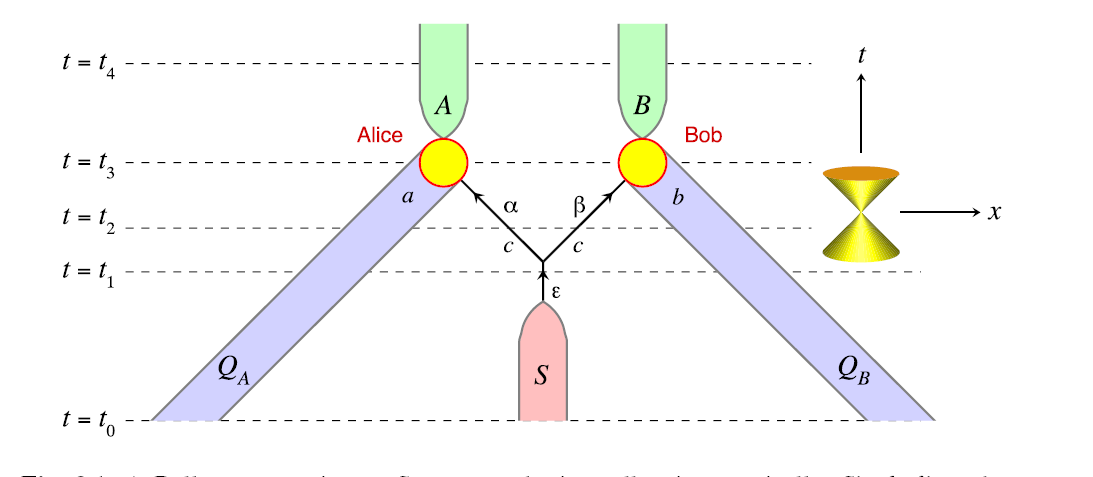
\includegraphics{images/img_3_1.png}
		}
		\caption{
		\label{i3.1} Эксперимент типа Белла. Пространство - горизонтальная ось, время - вертикальная ось. Одиночные линии обозначают путешествующие одиночные биты или кубиты; расширенные линии обозначают классическую информацию, переносимую миллионами бит. Свет распространяется под углом $45^\circ$, как указано световым конусом справа. Значение переменных: см. Текст}
	\end {center}
\end {figure}

Вернемся к делу. Эксперимент Белла показан на рис. \ref{i3.1}. В точке $S$ атом $\varepsilon$ подготовлен в нестабильном состоянии $J = 0$ при $t = t_1$, так что он может распадаться только в другое состояние $J = 0$, одновременно испуская два фотона, так что $\Delta J = 0$, и поэтому два фотона, $\alpha$ и $\beta$, должны находиться в запутанном состоянии $S_{tot} = 0$ при $t = t_2$.

После долгого путешествия, при $t = t_3$, фотон $\alpha$ обнаруживается наблюдателем $A$ (Алиса), а фотон $\beta$ обнаруживается $B$ (Бобом). В идеале наблюдатели используют поляризационный фильтр, ориентированный под углом $a$ (Алиса) и $b$ (Боб). Если фотон передается фильтром, он поляризован в направлении угла поляризационного фильтра, если он отражен, его поляризация становится ортогональной его углу. С обоих сторон фильтра есть детекторы, поэтому Алиса и Боб наблюдают, что один из двух их детекторов дает сигнал. Мы называем сигнал Алисы $A = + 1$, если фотон прошел фильтр, и $A = -1$ если он отразился, и аналогично определяем сигнал Боба.

Согласно квантовой теории, если A = 1, фотон Алисы поляризован в направлении $a$, поэтому фотон Боба также должен быть поляризован в этом направлении, и интенсивность света, проходящего через фильтр Боба, будет $\cos^2 (a - b)$. Следовательно, согласно квантовой теории, вероятность того, что B = 1, равна $\cos^2 (a - b)$. Тогда вероятность того, что B = -1, равна $\sin^2 (a - b)$, и те же рассуждения можно применять, если A = -1. Таким образом, ожидаемое значение произведения $AB$ оказывается равным

\begin{equation}\label{3.10}
	\langle A B\rangle=\cos ^{2}(a-b)-\sin ^{2}(a-b)=\cos 2(a-b)
\end{equation}
            
согласно квантовой механике.
 
Фактически, эти корреляционные функции теперь могут быть проверены экспериментально. Красивые эксперименты [2, 3] подтвердили, что корреляции хорошо согласуются с уравнением (\ref{3.10}).

Идея, высказанная Беллом, состоит в том, что невозможно воспроизвести эту сильную корреляцию между полученными данными А и В в любой теории, где классическая информация передается от атома $\varepsilon$ Алисе (А) и Бобу (В). Все, что нужно предположить, это то, что атом излучает сигнал Алисе, и еще один - Бобу, относительно поляризации испускаемых фотонов. Это может быть информация о том, что оба фотона $\alpha$ и $\beta$ поляризованы в направлении $c$. Поскольку эта информация передается задолго до того, как Алиса или Боб решили, как ориентировать свои поляризационные фильтры, очевидно, что сигналы в $\alpha$ и $\beta$ не должны зависеть от этого. Алиса и Боб могут свободно выбирать поляризаторы.

Тогда корреляции напрямую приводят к противоречию, независимо от природы классических сигналов. Противоречие достигается следующим образом. Рассмотрим два варианта, которые может сделать Алиса: выбрать углы $a$ или $a '$. Точно так же Боб может выбирать между углами $b$ и $b'$. Каким бы ни был сигнал, который несут фотоны, он должно повлечь за собой ожидаемое значение для четырех наблюдений, которые могут быть сделаны: Алиса наблюдает $A$ или $A'$ в обоих случаях, а Боб наблюдает $B$ или $B'$. Если и Алиса, и Боб проводят большое количество наблюдений, каждый раз используя один из двух своих вариантов, они могут впоследствии сверить данные и измерить средние значения $AB$, $A'B$, $AB'$ и $A'B'$. Они рассчитывают среднее

\begin{equation}\label{3.11}
	S=\langle A B\rangle+\left\langle A^{\prime} B\right\rangle+\left\langle A B^{\prime}\right\rangle-\left\langle A^{\prime} B^{\prime}\right\rangle
\end{equation}

и смотрят, как оно зависит от углов поляризации $a$ и $b$.

Теперь предположим, что каждый раз, когда испускаются фотоны, они имеют четко определенные значения для $A$,$ A '$, $B$ и $B'$. Независимо от того, какие сигналы передаются фотонами, при каждом измерении эти четыре члена будут принимать значения $\pm 1$, но все они никогда не смогут внести вклад в величину $S$ с одним и тем же знаком (из-за знака минус в (\ref{3.11})), из-за этого легко заметить, что $S$ всегда $\pm 2$, и поэтому его среднее значение будет подчиняться:

\begin{equation}\label{3.12}
	|\langle S \rangle| \leq 2;
\end{equation}
            
Эта современная версия оригинального наблюдения Белла называется неравенством Клаузера-Хорна-Шимон-Холта (CHSH) [20, 78]. Однако, если мы выберем углы

\begin{equation}\label{3.13}
	a = 22.5^\circ,\quad a'= 22.5^\circ,\quad b = 0 ^\circ,\quad b' = 45^\circ, 
\end{equation}
                                                     
затем, согласно формуле (\ref{3.10}) квантовая механика дает ожидаемое значение

\begin{equation}\label{3.14}
	S = 3cos (45^\circ) \cos 135^\circ = 2 \sqrt 2> 2.
\end{equation}

Как так получается? По-видимому, квантовая механика не дает явных значений $\pm 1$ для измерений $A$ и $A '$; она только дает значение фактически измеренной величины, которая в каждом случае является либо $A$, либо $A '$, а также либо $B$, либо $B'$. Если Алиса измеряет $A$, она также не может измерить $A '$, потому что оператор для $ A'$ не коммутирует с $A$; поляризаторы различаются на угол $45 ^\circ$, и фотон поляризован вдоль одного из углов, который является суперпозицией фотона, поляризованного под другим углом, и фотон, поляризованный ортогонально этому. Таким образом, квантовый результат полностью соответствует предписаниям Копенгагена, но кажется, что он не может быть реализован в локальной теории скрытых переменных.

Мы говорим, что, если $A$ измеряется фактически, измерение $A '$ является контрфактуальным, что означает, что мы представляем себе измерение $A'$, но на самом деле мы не можем это сделать, точно так же, как мы не можем измерить положение, если мы уже выяснили, какой именно импульс имеет частица. Если две наблюдаемые не коммутируют, одна может измерить другую, но измерение другой контрфактуально.

Действительно, в использованных аргументах предполагалось, что теория скрытых переменных должна позволять наблюдателю фактически выполнять контрфактуальные измерения. Это называется определенностью. Говорят, что локальные теории скрытых переменных, допускающие контрфактические наблюдения, имеют локальную определенность. Квантовая механика запрещает локальную контрфактуальную определенность.

Однако применять термины «определенность» или «реализм» для возможности выполнения контрфактивных наблюдений не очень правильно. «Реализм» должен означать, что на самом деле просто что-то происходит - не суперпозиция вещей; что-то происходит наверняка, а что-то еще не происходит. Это не то же самое, что сказать, что и Алиса, и Боб всегда могут изменить свои поляризационные углы, не допуская каких-либо изменений в других местах [85].

Именно здесь вводится понятие «свободная воля» [22, 23], часто являющееся неточным. Беллом было сделано предположение, часто умалчиваемое многими его последователями, заключающееся в том, что и Алиса, и Боб должны иметь «свободную волю» для изменения своих настроек в любой момент, не обращаясь к настройкам в системе $S$, которые производит нестабильный атом. Если бы это допускалось в теории скрытых переменных, мы бы получили локальную контрфактуальную определенность, что было исключено.

Суть аргумента, который теперь следует, на самом деле была поднята раньше. Формулировка C. H. Brans [14] в основном верна, но мы добавим дополнительный момент, который будет называться «законом сохранения онтологии» (разд. \ref{ch3.7.1}), чтобы указать, почему нарушение теоремы Белла не требует "абсурдной физики".

Как мы можем отказать Алисе и/или Бобу в их свободной воле? Что ж, именно в теории детерминированных скрытых переменных Алиса и Боб могут изменить свое мнение о настройке своих поляризаторов, если их мозг подчиняется неким законам, действующим в прошлом, и, нравится это или нет, действия Алисы и Боба определяются законами физики [118], даже если это только локальные законы. Их решения, по логике вещей, уходят своими корнями в далекое прошлое, начиная с Большого взрыва. Так почему мы должны верить, что они могут делать контрфактивные наблюдения?

Этот аргумент обычно опровергается тем, что корреляции между фотонами c распадающегося атома и настройками $a$ и $b$, выбранными Алисой и Бобом, должны быть удивительно сильными. Гигантский сложный алгоритм мог заставить Алису и Боба принимать свои решения, и все же распадающийся атом задолго до того, как Алиса и Боб применили этот алгоритм, знал о результате. Это называется «заговор», и считается, что заговоры это «отвратительно». «Лучше прекратить заниматься физикой, чем поверить в такую странную вещь», - шутят некоторые исследователи.\footnote{Это скорее вопрос психологии (нейробиологии) нежели физики - \textit{прим. переводчика}}

В разделах \ref{ch3.7.1}, \ref{ch5.7.3} и \ref{ch10.3.3}, мы переходим к сути этой проблемы.

\subsection{The Mouse Dropping Function}\label{ch3.7}

Чтобы проиллюстрировать, насколько безумные результаты можно получить, была предложена отточенная версия эксперимента Белла: и Алиса, и Боб несут с собой мышь в клетке с едой.\footnote{Эта версия была выдвинута в дискуссии в блоге. К сожалению, я не помню, кто поднял ее, и я не могу найти его основа} Каждый раз, когда они хотят установить углы своих поляризаторов, они считают количество помета мыши. Если количество какулек четное, они выбирают один угол, если оно нечетное, они выбирают другой. "Теперь распадающийся атом должен заранее знать, сколько помета будет производить мышь. Разве это не отвратительно?"

Чтобы увидеть, что нужно для получения этого «отвратительного» результата, рассмотрим простую модель. Мы предполагаем, что существуют корреляции между совместными поляризациями двух запутанных фотонов, называемых $c$, и настройками, $a$ выбранными Алисой, и $b$, выбранными Бобом. Все эти углы взяты в интервале [0, $180^\circ$]. Определим функцию $W(c | a, b)$ как условную вероятность того, что оба фотона поляризованые в направлении $c$, дают $a$ и $b$. Предположим, что результат Алисы будет $A = + 1$, как только ее «онтологический» фотон принимает состояние $| a-c | < 45^\circ$ или $ > 135^\circ$, в противном случае $A = 1$. Для измерения Боба, заменяя $a\leftrightarrow b$ и наоборот, мы предполагаем то же самое. Все будет периодическим по $a$, $b$ и $c$ с периодом $\pi (180^\circ)$.

Разумно ожидать, что $W$ зависит только от относительных углов $c-a$ и $c-b$:

\begin{equation}\label{3.15}
	W (c | a, b) = W (x-a, c-b); \quad  \int^\pi_0 dc\, W (c-a, c-b) = 1.
\end{equation}

Введите функцию сигнум $s_{(\varphi)}$ следующим образом:

\begin{equation}\label{3.16}
	s_{(\varphi)} \equiv \operatorname{sign}(\cos (2 \varphi)) ; \quad A=s_{(c-a)}, \quad B=s_{(c-b)}
\end{equation}
                            
Ожидаемое значение произведения $AB$


\begin{equation}\label{3.17}
	\langle A B\rangle=\int \mathrm{d} c\, W(c | a, b) s_{(c-a)} s_{(c-b)}
\end{equation}
           
Как выбрать $W$, чтобы воспроизвести квантовое выражение (\ref{3.10})?

Ведем новые переменные:

\begin{equation}\label{3.18}
	x=c-\frac{1}{2}(a+b), \quad z=\frac{1}{2}(b-a), \quad W=W(x+z, x-z)
\end{equation}
           
Квантовая механика требует, чтобы


\begin{equation}\label{3.19}
	\int_{0}^{\pi} \mathrm{d} x W(x+z, x-z) s_{(x+z)} s_{(x-z)}=\cos 4 z
\end{equation}

Записывая

\begin{equation}\label{3.20}
	s_{(x+z)} s_{(x-z)}=\operatorname{sign}(\cos 2(x+z) \cos 2(x-z))=\operatorname{sign}(\cos 4 x+\cos 4 z)
\end{equation}

мы видим, что уравнения являются периодическими с периодом $\pi / 2$, но при более внимательном рассмотрении мы видим, что обе стороны уравнения (\ref{3.19}) меняют знак, если $x$ и $z$ сдвинуты на величину $\pi / 4$. Поэтому сначала пробуем решения с периодичностью $\pi / 4$. Кроме того, имеем место симметрия $x \leftrightarrow — x$, $z \leftrightarrow — z$.

Уравнение (\ref{3.19}) содержит больше неизвестных, чем уравнений, но если мы предположим, что $W$ зависит только от $x$, но не от $z$, тогда уравнение может быть легко решено. Дифференцируюя уравнение (\ref{3.19}) по $z$, получаем внутри интеграла  дельта-функцию Дирака, и записываем результат:

\begin{equation}\label{3.21}
	4 \int_{0}^{\pi / 4} W(x) \mathrm{d} x(-2 \delta(x+z-\pi / 4))=-4 \sin 4 z, \quad \text { if } \quad 0<z<\frac{1}{4} \pi
\end{equation}

(каждая из четырех частей интеграла в (\ref{3.19}) дает одинаковый вклад, следовательно, первый множитель $= 4$). Таким образом получим

\begin{equation}\label{3.22}
	W(c | a, b)=W(x+z, x-z)=\frac{1}{2}|\sin 4 x|=\frac{1}{2}|\sin (4 c-2 a-2 b)|
\end{equation}

Это также дает нормализованное 3-точечное распределение вероятностей,

\begin{equation}\label{3.23}
	W(a, b, c)=\frac{1}{2 \pi^{2}}|\sin (4 c-2 a-2 b)|
\end{equation}

Из проверки мы находим, что эта корреляционная функция $W$ действительно приводит к квантовому выражению (\ref{3.10}). Мы могли бы назвать это «функцией мышинных какулек» (см. Рис. \ref{i3.2}). Если Алиса хочет выполнить контрфактивное измерение, она изменяет угол $a$, в то время как $b$ и $c$ остаются нетронутыми. При этом она выбирает конфигурацию, которая является менее вероятной или более вероятной, чем конфигурация, которую она имела ранее.

\begin{figure}[ht] % вставляем рисунок
	\begin{center}
		\scalebox{0.4}{
		   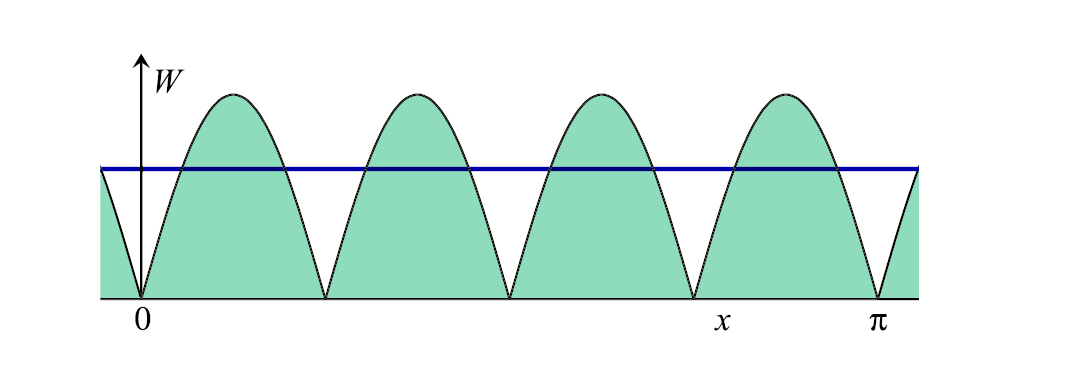
\includegraphics{images/img_3_2.png}
		}
		\caption{
		\label{i3.2}Функция помета мыши, уравнение (\ref{3.23}). По горизонтали переменная $x = c - \frac 1 2 (a + b)$. Усреднение по любой из трех переменных $a$, $b$, или $c$ дает тот же результат, что и плоская линия, тогда корреляции исчезают}
	\end {center}
\end {figure}

Имея в виду о возможной интерпретации вероятностей Борна, как это выражено в разд. \ref{ch3.5} и \ref{ch4.3}, приходим к выводу, что конфигурация начальных состояний, когда мышь Алисы производила различное количество помета, может быть более вероятной или менее вероятной, чем состояние, которое она имела до этого. Мы узнали, что в квантовой механике это приемлемо. Если же мы обсуждаем это с точки зрения основополагающей детерминированной теории, то, похоже, с этим возникают проблемы.

\subsubsection{Сохранение онтологии и скрытая информация}\label{ch3.7.1}

Фактически, основная мысль приведенных выше выкладок, заключается в том, что даже в детерминированной теории, подчиняющейся локальным уравнениям, конфигурации шаблонных состояний могут иметь нетривиальные пространственно-подобные корреляции. Как известно,  это происходит во многих физических системах. Жидкость, близкая к ее термодинамической критической точке, демонстрирует явление, называемое критической опалесценцией, обусловленной большими колебаниями локальной плотности.\footnote{Опалесценция - физ. явление рассеяния света мутной средой, обусловленное её оптической неоднородностью; } Это означает, что корреляционные функции плотности нетривиальны на относительно больших пространственных расстояниях. Это не влечет за собой нарушения теории относительности или любого другого принципа в физике, такого как причинность; это нормальное явление. Жидкость не должна быть квантовой жидкостью, чтобы показать критическую опалесценцию.

Эффект помета мыши кажется загадочным, поскольку в некотором смысле он отрицает, что Алиса, Боб и их мыши имеют «свободную волю». Что такое «свободная воля»? Мы предпочитаем математическое определение, а не эмоциональное (см. Раздел \ref{ch3.8}), и мы также вернемся к этому вопросу в нашем последующем обсуждении в разделах. \ref{ch10.2} и \ref{ch10.3}. Все, что мы можем выдвинуть сейчас, это то, что кишки мышей также подчиняются закону сохранения энергии, импульса и момента импульса, как и все в мире, потому что это общие законы. В нашей теории «скрытой переменной» к этому должен быть добавлен общий закон: онтологическое состояние развивается в онтологическое состояние; суперпозиции превращаются в суперпозиции. Если помет мыши является онтологическим в одном описании и неэффективным в другом, то исходное состояние, из которого оно произошло, также было онтологическим или контрфактуальным, соответственно. В этом утверждении не должно быть ничего загадочного.

Однако в этом аргументе есть проблемный элемент, который состоит в том, что каким-то образом запутанные фотоны, покидающие источник, уже несут информацию о настройках, которые будут использоваться Алисой и Бобом. Они сами не сообщают нам настройки, но несут информацию о корреляционной функции этих настроек. Таким образом, нелокальная информация о будущем уже присутствует в «скрытых» онтологических данных фотонов, информация, которая исчезает, когда мы перефразируем то, что происходит в терминах стандартных квантово-механических описаний. Таким образом, в онтологическом описании происходящего есть нетривиальная информация о будущем. Мы утверждаем, что, пока эта информация подчиняется строгому закону сохранения - закону сохранения онтологии, как описано выше, - здесь нет противоречия, но мы подозреваем, что это может пролить свет на идею супердетерминизма.

На самом деле, существует даже менее тривиальное соглашение, чем помет мыши, с помощью которого Алиса и Боб могут принимать свои решения. Они могли бы одновременно отслеживать флуктуации света, вызванные светом, исходящим от разных квазаров в противоположных точках неба [38], и использовать их для определения настроек $a$ и $b$ своих фильтров. Эти квазары, обозначенные как $Q_A$ и $Q_B$ на рис. \ref{i3.1}, могли испускать свои фотоны вскоре после Большого взрыва, в момент времени $t = t_0$ на рисунке, когда они находились на расстоянии миллиардов световых лет друг от друга. Колебания этих квазаров также должны подчиняться формуле мышинных каках (\ref{3.22}). Как такое может быть? Единственное возможное объяснение - это то, что предлагает теория инфляции ранней вселенной: эти два квазара вместе с распадающимся атомом имеют общее прошлое, и поэтому их свет коррелирован.
Обратите внимание, что корреляция, генерируемая распределением вероятностей (\ref{3.23}), является подлинной корреляцией трех тел. Интегрирование по любой из трех переменных дает плоское распределение. Квазары коррелируют только через состояние, в котором находится распадающийся атом, но не напрямую друг с другом. Это явно таинственная корреляция, но она не противоречит тому, что мы знаем о законах физики, см. Замечания в конце секц. \ref{ch20.6} и \ref{ch20.7} в части II.

На самом деле, эти космические корреляции должны быть огромными: кто знает, где еще во вселенной некоторые инопланетные Алисы и Бобы проводят эксперименты, используя те же квазары...

\subsection{Свободная воля и инверсия времени}\label{ch3.8}

Понятие «свободная воля» может сбивать с толку. В некоторых случаях дискуссия кажется граничащей с религиозной. Должно быть совершенно ясно, что теории Природы, обсуждаемые в этой книге, не имеют ничего общего с религией, и поэтому мы должны сформулировать более конкретно то, что подразумевается под «свободной волей».

Идея, лежащая в основе того, что часто называют «свободной волей», в принципе чрезвычайно проста. Представьте, что у нас есть модель, которая описывает то, что происходит в Природе, например, мысленный эксперимент, для которого Белл и CHSH написали свои неравенства. Предположим, что мы описали распадающийся атом, испускающий два фотона, в терминах некоторых кинематических переменных. Все, что мы хотим знать, это то, как отреагирует система в модели, если мы сделаем небольшое изменение настроек, выбранных Алисой, оставив Боба и запутанные фотоны нетронутыми. Как бы поток информационных носителей взаимодействовал, чтобы привести к результатам, которые нарушают это неравенство?

Мы знаем, что не существует божественного создателя модели, который мог бы делать такие изменения, но это не главное. Мы знаем, что, собственно говоря, у Боба нет свободы воли, чтобы вносить изменения самостоятельно. Но что скажет модель? Чего действительно можно ожидать от теории, так это того, что:

\textit{теория предсказывает, как ее переменные однозначно эволюционируют из любого выбранного начального состояния.}

Предположим, что в эксперименте Белловского типа мы начинаем с конфигурации с заданными параметрами фильтров $a$ и $b$ Алисы и Боба. Мы видим запутанные частицы, движущиеся от источника к двум детекторам. Нам нужна наша модель, чтобы прописать, что происходит, когда мы смотрим на состояние, которое было изменено, как описано выше. Таким образом, на самом деле это \textit{свобода выбора начального состояния в любое время $t$}, которую можно ввести в теорию.

Обратите внимание, что это подразумевает, что можно игнорировать вопрос, как эти состояния могли эволюционировать из конфигураций в прошлом. Весь аргумент «свободной воли» предполагает, что нам не нужно проверять, какие модификации потребовались бы в прошлых событиях, чтобы реализовать новую модификацию. Независимо от того, что это за состояние, теория должна давать прогноз. Белл вывел свои неравенства для результатов различных начальных состояний, которые он выбрал, и эти неравенства, по-видимому, нарушаются квантовой механикой.

Мы вывели в разд. \ref{ch3.7} что для воспроизведения квантово-механического результата, вероятности настроек $a$, $b$ и $c$ должны быть коррелированы, а корреляционная функция, связанная с одной простой моделью, была рассчитана. Здесь мы видим, как, в принципе, понятию свободной воли, данному выше, можно противопоставить:

\textit{Внесение изменений в заданные значения кинетических переменных порождает изменение и вероятностей.}

Найденная нами корреляционная функция описывает 3-точечные корреляции. Все двойные корреляции исчезают.

Теперь ситуацию можно дополнительно прояснить, если мы воспользуемся важным свойством, которое уравнение Шредингера разделяет с классическими уравнениями Ньютона: микроскопические законы могут быть решены задом наперед.

Скажем только Алиса, изменила свои настройки, и фотоны остались без изменений. Тогда мы можем прийти к конфигурации, которая, по-видимому, нарушает неравенство Белла или неравенство CHSH.\footnote{То есть в статистическом смысле; были и более продуманные конструкции состояний, которые приводили бы к конфигурациям, которые полностью исключались при написании в терминах скрытых переменных.} В более ранних дискуссиях о супердетерминизме было заявлено, что Алиса не имеет «свободной воли», чтобы сделать это, но теперь мы говорим: возможно, нет, но мы, безусловно, можем позволить себе изучить полученное состояние, и спросить какой была физическая структура в прошлом, решая микроскопические уравнения назад во времени.

И теперь нетрудно увидеть, что тогда произойдет. Квантовое состояние запутанных фотонов больше не будет подготовлено изначально: фотоны улетающие от Алисы (назад во времени) теперь имеет другую поляризацию. Исходное состояние, в котором суммарный спин двух фотонов был равен нулю ($S$-состояние), теперь будет частично содержать состояние $D$, с суммарным спином $s = 2$. Таким образом, выбирая различные настройки, Алиса или Боб изменили состояния фотонов, которые они обнаруживают. Далее состояние $s = 2$ возвращается назад в прошлое, и мы видим не распад атома, а гораздо менее вероятное состояние отскока фотонов от атома, отказывающегося выполнить предполагаемый процесс распада назад во времени. Термодинамически, это гораздо менее вероятное начальное состояние; это контрфактическое начальное состояние.

Это контрфактическое начальное состояние будет полностью законным с точки зрения микроскопических законов физики, но, вероятно, совсем не с точки зрения макроскопических законов, в частности термодинамики. Этот аргумент показывает, что теорема Белла требует больше скрытых допущений, чем обычно полагается: квантовая теория противоречит классической теории только в том случае, если мы предположим, что «контрфактическая модификация» не нарушает законы термодинамики.

В наших моделях мы должны предполагать, что это так. Неизбежно, более «вероятная» модификация настроек действительно превращает фотонное состояние в другое. На первый взгляд это кажется странным: модификация была сделана в одной из настроек, а не в приближающихся фотонах. Однако мы должны признать, что фотоны, описанные на языке квантовой механики, находятся в шаблонных состояниях; онтологические состояния, образующие ортонормированное множество, должны включать в себя гораздо больше онтологических степеней свободы, чем только эти два фотона, чтобы оставаться ортонормированными.

Отметим, что, наконец, здесь установлена причина нарушения неравенств CHSH. В итоге: понятие «свободной воли» должно быть заменено понятием, что полезная модель Природы должна давать правильные прогнозы относительно того, что происходит для любого данного начального состояния (свобода выбора начального состояния), тогда как контрфактивное начальное состояние рассматриваемое в эксперименте Белла приводит к тому, что исходные запутанные фотоны получают примесь со спином 2, что значительно подавляет вероятность этого состояния.
В секциях \ref{ch4.2} и \ref{ch4.3} мы увидим, что квантово-механические вероятности действительно можно проследить до вероятностей в начальном состоянии. Поэтому, когда в момент времени $t = t_3$ амплитуда оказывается низкой, а вероятность Борна мала, это на самом деле может быть связано с меньшей вероятностью выбранного начального состояния при $t = t_1$. Состояние $spin = 2$ для распадающегося атома имеет гораздо меньшую вероятность, чем состояние $spin = 0$.


\end{document}